\chapter{Data Transmisi}

\section{Konsep dan Terminologi}

\section{Transmisi Data Analog dan Digital}

\section{Gangguan Transmisi}

\section{Kapasitas Kanal}

Kita sudah mempelajari bahwa terdapat berbagai jenis gangguan (impairment) yang dapat merusak sinyal. Sejauh mana gangguan tersebut dapat membatasi data rate pada data digital. Data rate maksimum yang dapat dicapai disebut kapasitas kanal (channel capacity).

Terdapat empat konsep yang perlu dipahami:
\begin{enumerate}
	\item Data Rate: Laju dimana data dapat dikomunikasikan dengan satuan bps atau bits per second.
	\item Bandwidth: Bandwidth dari sinyal yang ditransmisikan yang dibatasi oleh transmitter atau sifat media transmisinya
	\item Noise: Level rata-rata dari noise sepanjang jalur transmisi
	\item Error rate: Rate dimana error dapat terjadi. Error di sini adalah ketika yang diterima adalah 1 sedangkan yang dikirimkan adalah 0 atau sebalikn
\end{enumerate}

Permasalah yang dialami adalah semakin besar bandwidth maka semakin besar ongkosnya. Sehingga semua kanal transmisi memiliki bandwidth yang terbatas. Batasan ini disebabkan oleh sifat-sifat fisi dari media transmisinya atau dari transmitter-nya untuk menghindari terjadinya interferensi dari sumber lain. Berdasarkan hal ini maka sepatutnya kita memakai bandwidth seefisien mungkin. Jika di dalam data digital maka kita akan memakai data rate sebesar mungkin pada batas error rate dari bandwidth yang tersedia. Kemudian kendala terbesar untuk mencapai efisiensi ini adalah noise.


\subsection{Nyquist Bandwidth}

Pertama, anggaplah ada sebuah kanal transmisi yang bebas dari noise. Pada kondisi seperti ini, keterbatasan dari data rate adalah bandwidth dari sinyal itu sendiri. Berdasarkan Nyquist, persamaan dari keterbatasan ini adalah sebagai berikut. Jika laju transmisi sinyal adalah $ 2B $, maka sinyal dengan frekuensi tidak lebih besar dari $ B $ sudah cukup untuk membawa laju sinyal. Begitu juga sebaliknya, jika diketahui bandwidth sebesar $ B $, maka laju sinyal tertinggi yang dapat dibawa adalah $ 2B $.

Jika sinyal yang akan ditransmisikan adalah biner (2 level tegangan), maka data rate yang dapat didukung oleh $ B $ Hz adalah $ 2B $ bps. Misalkan, jika menggunakan empat level tegangan maka setiap elemen sinyal dapat direpresentasikan sebagai 2 bits. Dengan multilevel signaling, persamaan Nyquist menjadi

\begin{equation} \label{pers.nyquist}
	C = 2B \log_2 M
\end{equation}

Dimana $ M $ adalah banyaknya sinyal diskret atau level tegangan.

Dari Persamaan \ref{pers.nyquist} dapat kita simpulkan bahwa data rate dapat ditingkatkan dengan meningkatkan jumlah perbedaan dari elemen sinyalnya / banyaknya level tegangannya. Namun dengan meningkatkan elemen sinyal maka akan membuat beban dari receiver juga meningkat.

Misal, diketahui bahwa data digital akan ditransmisikan menggunakan modem. Bandwidth yang digunakan adalah 3100 Hz. Maka Nyquist capacity ($ C $) dari kanalnya adalah $ 2B $ = 6200 bps. Jika $ M $ = 8, maka $ C $ menjadi 18.600 bps dengan bandwidth sebesar 3100 Hz.

\subsection{Shannon Capacity Formula}

Berdasarkan persamaan Nyquist sebelumnya, kita mengetahui bahwa dengan meningkatkan bandwidth sebesar 2 kalinya maka data rate juga akan meningkat sebesar 2 kalinya. Sekarang asumsikan bahwa terdapat noise dan error rate. Dengan adanya noise maka 1 atau lebih bits akan rusak. Jika data rate meningkat maka bits semakin pendek. Akibatnya akan lebih banyak bits yang akan dipengaruhi oleh pattern/pola dari noise tersebut seperti yang ditunjukkan oleh Gambar \ref{fig.aklibat_noise}.

\begin{figure}
	\centering
	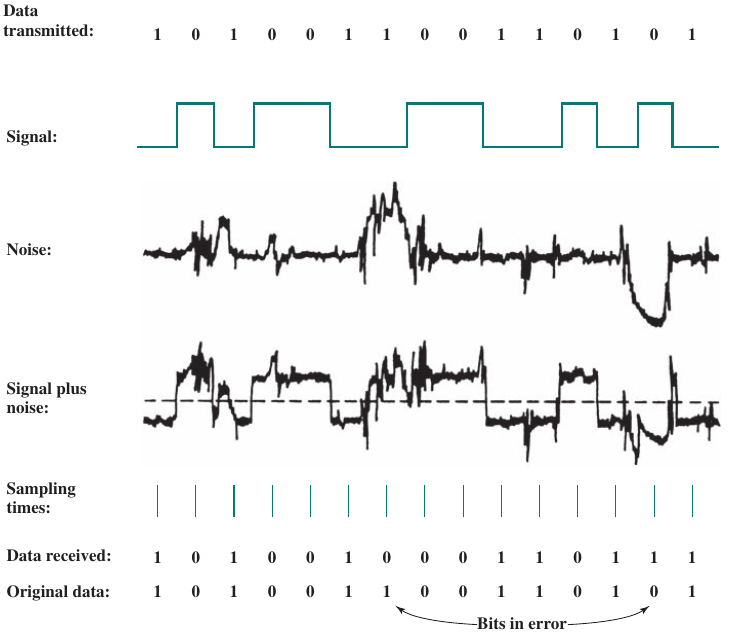
\includegraphics[width=1\linewidth]{gambar/3.4.gambar.3.15.akibat_noise_pada_sinyal_digital}
	\caption{Akibat dari Noise terhadap Sinyal Digital}
	\label{fig.aklibat_noise}
\end{figure}

Jika data rate ditingkatkan maka lebih banyak bits yang akan terjadi selama interval noise spike-nya, sehingga lebih banyak error yang terjadi. Untuk level noise tertentu, dengan kekuatan sinyal yang lebih besar dapat meningkatkan kemampuan untuk menerima data dengan benar meskipun ada noise. Parameter yang menyatakan hal ini adalah \textbf{signal-to-noise-ratio} (SNR) yaitu rasio dari daya sinyal terhadap daya dari noise. Biasanya SNR diukur di receiver dan dalam bentuk desibel

\begin{equation}
	\text{SNR}_{\text{dB}} = 10 \log_{10} \frac{\text{signal power}}{\text{noise power}}
\end{equation}

Semakin tinggi nilai SNR maka semakin tinggi kualitas sinyal dan semakin sedikit repeater yang dibutuhkan.